\subsection{Artificial Neural Network}
\label{subsec:ann}

\begin{figure}
    \begin{subfigure}{.5\textwidth}
        \centering
        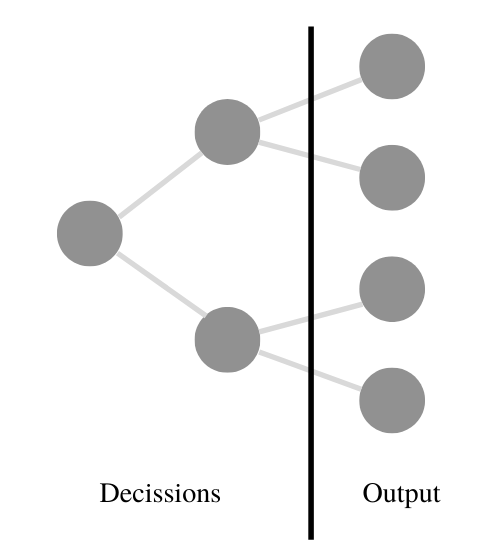
\includegraphics[width=.7\linewidth]{pics/Decission Tree.png}
        \caption{Decision tree}
        \label{fig:decission_graphic}
    \end{subfigure}%
    \begin{subfigure}{.5\textwidth}
        \centering
        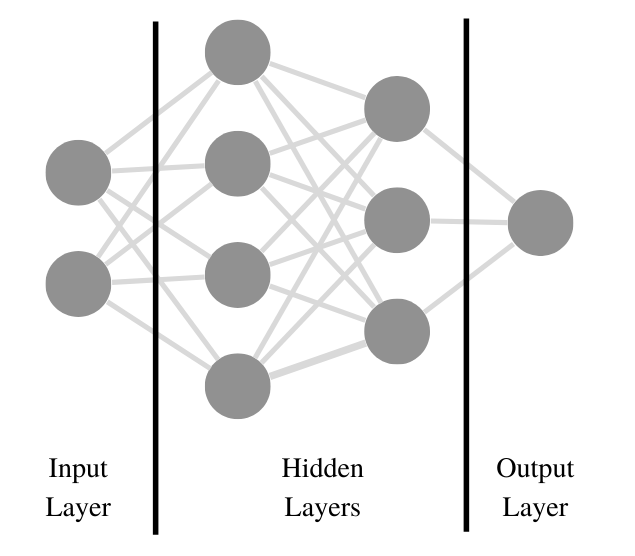
\includegraphics[width=.9\linewidth]{pics/Neural Network.png}
        \caption{Neural network}
        \label{fig:nn_graphic_representation}
    \end{subfigure}
    \centering
    \caption{A graphical representation of the models}
    \label{fig:graphical_representation}
\end{figure}

The second machine learning method we will use in this thesis is an artificial neural network. Because the neural network works in a very different way than the XGBoost model, it would diversify the selection of models in this thesis. The neural network for regression purposes was proposed by \cite{Specht1991ANetwork}. A neural network is a structure that uses one or multiple hidden layers to make a non-linear transformation which is loosely based on biological neural systems. The network consists of multiple layers performing operations and together they form the network. The three different types of layers in a neural network are the input layer, the hidden layers and the output layer. The input layer consists of the inputs $X = \{x_1, x_2, ..., x_d\}$ which are the regressors. There can only be one input layer. The hidden layers form linear combinations between the input layer, other hidden layers and the output layer. These linear combinations together will make a non-linear function. There can be multiple hidden layers. The output layer is the final layer where the dependent variables $Y = \{y_1, ..., y_d\}$ are formed. There can only be one output layer.\\

A graphical representation of these layers in a simplified form can be found in figure \eqref{fig:nn_graphic_representation}. Between the layers, the function $f(x) = w_2 g(w_1^T x + b_1) + b_2$ is used. Where $\{w_1, w_2, b_1, b_2\} = \theta, w_1 \in \mathbb{R}^n \text{ and } w_2, b_1, b_2 \in \mathbb{R}$ are the function parameters. The function $g(\cdot): \mathbb{R} \to \mathbb{R}$ is the activation function defined in \eqref{eq:nn_activationfunction}
\begin{equation}
\label{eq:nn_activationfunction}
    g(z) = \frac{e^z - e^{-z}}{e^z + e^{-z}}
\end{equation}
To be able to estimate the network, backpropagation is used which tries to decrease the Loss function. In every iteration, after the Loss function of the output layer is calculated, the backpropogation makes backward passes which updates the previous layers with new weights to decrease the loss function. To calculate the updated weights the L-BFGS function is used \citep{Liu1989OnOptimalization}.
\begin{equation}
    Loss(\hat{y}, y, W) = \frac{1}{2n} \sum\limits_{i=0}^n ||\hat{y}_i - y_i||^2_2 + \frac{\alpha}{2n} ||W||^2_2
\end{equation}
This thesis will use the Scikit-learn implementation of the neural model described by \cite{Pedregosa2011Scikit-learn:Python}.\\

There will also be a multivariate implementation of the Neural Network where the data is broken down by skill level as is also done with the VARIMAX model. 